\documentclass[a4paper, 11pt]{article}
\usepackage[english]{babel}
\usepackage[top=2cm,bottom=2cm,left=2cm,right=2cm]{geometry}
\usepackage[utf8]{inputenc}
\usepackage{import}
\usepackage{float}
\usepackage{subfigure}
% \usepackage{subfig}
\usepackage[pdftex]{graphicx}
% \usepackage{graphicx}
\usepackage{amssymb,amsmath,amsthm,amsfonts}
\usepackage{xspace}
\usepackage{tabularx}
\usepackage{indentfirst}
\usepackage{wrapfig,booktabs}
%\usepackage[small]{caption}
% \usepackage{subcaption}
\usepackage{eucal}
\usepackage{eso-pic}
\usepackage{hyperref}
\usepackage{url}
\usepackage{booktabs}
\usepackage{afterpage}
\usepackage{parskip}
\usepackage{listings}
\usepackage{fancyhdr}
\usepackage{textcomp}
\usepackage{cite}
\usepackage{multirow,multicol}
\usepackage{setspace}
\usepackage[version=4]{mhchem}
\usepackage{nicefrac}
\usepackage{siunitx}

\usepackage{caption}
\captionsetup{tableposition=top,font=small,width=0.8\textwidth}
%\usepackage[table]{xcolor}
\usepackage[arrowdel]{physics}
\usepackage{mathtools}
\usepackage{tablefootnote}
\usepackage{enumitem}

\setlist[description]{font={\scshape}} %style=unboxed,style=nextline
\usepackage{floatflt}
\usepackage{commath}
\usepackage{bm}
\usepackage{ifthen}
\usepackage{comment}
\usepackage[colorinlistoftodos,textsize=tiny]{todonotes}

\newcommand{\overbar}[1]{\mkern 1.5mu\overline{\mkern-1.5mu#1\mkern-1.5mu}\mkern 1.5mu}
\let\oldfrac\frac
\renewcommand{\frac}[3][d]{\ifthenelse{\equal{#1}{d}}{\oldfrac{#2}{#3}}{\nicefrac{#2}{#3}}}


\begin{document}

\title{Quantum Optics Lab report}
\author{Alessandro Lovo}

\maketitle

\begin{abstract}
  In this report, using the same experimental apparatus, three experiments regarding the quantum entanglement of photons will be performed: Entangled Quantum Key Distribution, Bell Inequality Violation and Quantum Tomography.
\end{abstract}


\section{Experimental apparatus}
  \begin{figure}[H]
    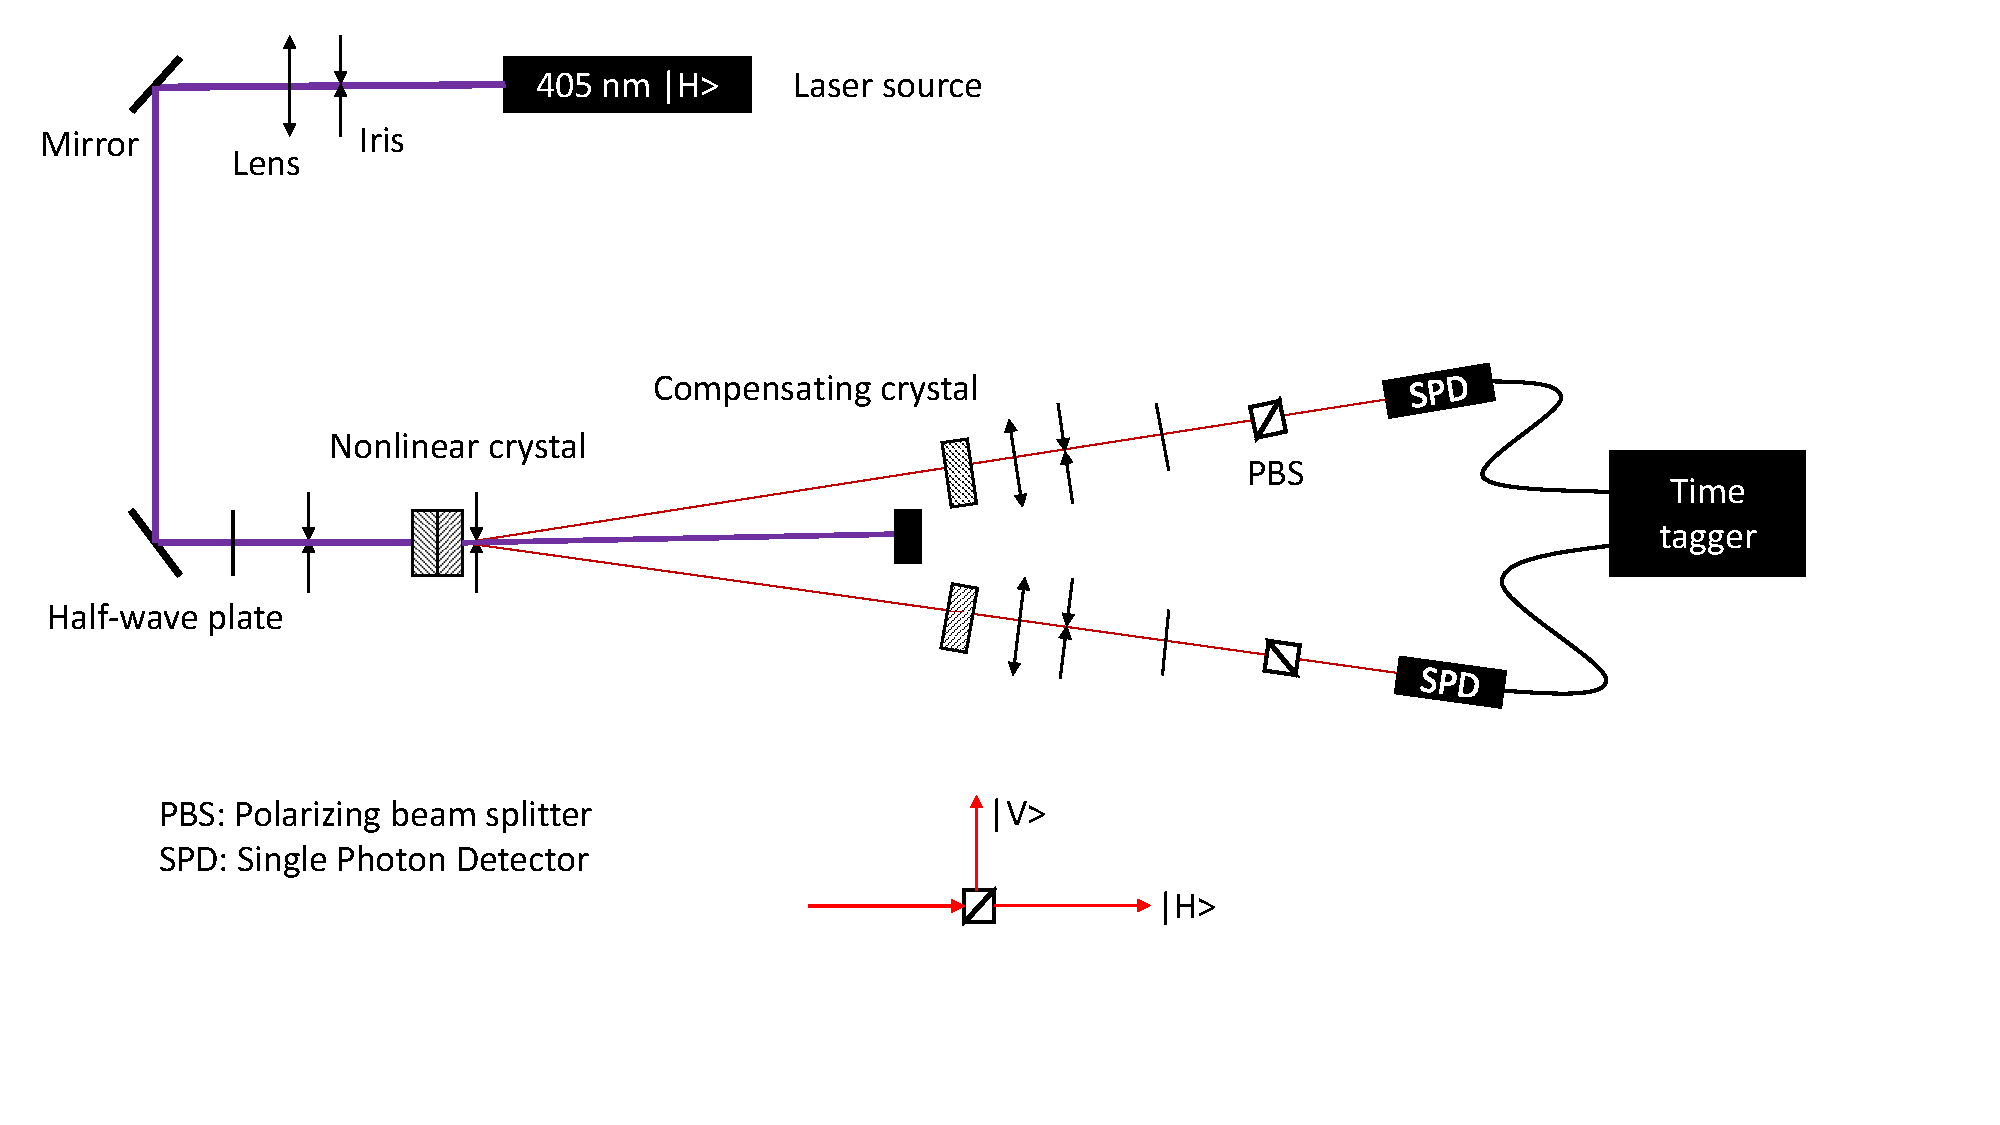
\includegraphics[width=1.0\textwidth]{img/apparatus.pdf}
    \caption{Schematics of the experimental apparatus.}
    \label{fig:apparatus}
  \end{figure}
  The schematics of the experimental apparatus are reported in fig \ref{fig:apparatus}: the source is a 405 \si{\nano\meter} laser whose beam is focused onto a nonlinear type II crystal obtained by sticking together two type I crystals with perpendicular optical axes. The laser emits light horizontally polarized ($\ket{H}$) and the two nonlinear crystals have a small chance ($\sim 10^{-7}$) of converting a photon into a pair of photons: if $\ket{V}$ is the vertical polarization, the conversion reads as:
  \begin{gather*}
    \ket{H} \xrightarrow[]{\text{crystal 1}} \ket{VV} \quad
    \ket{V} \xrightarrow[]{\text{crystal 2}} \ket{HH}
  \end{gather*}
  Using the first half-wave plate the polarization of the beam is rotated to the diagonal state $\ket{D} = \frac{\ket{H} + \ket{V}}{\sqrt{2}}$, so when it impinges on the two crystals the exiting pair is in the entangled state $\ket{\phi^+} = \frac{\ket{HH} + \ket{VV}}{\sqrt{2}}$. However since the conversion is due to two type I crystals, in order to not be able to distinguish which one did the conversion, two compensating crystals are introduced on the optical path. After some focusing, the two beams hit the measuring device: a half-wave plate, a polarizing beam splitter (PBS) and a single photon detector (SPD).
  By tuning the angle $\alpha$ of the half-wave plate it is possible to measure any linear polarization $\ket{\theta} = \cos{\theta}\ket{H} + \sin{\theta}\ket{V}$ with the simple relation $\theta = 2\alpha$.
  The signals of the SPDs are sent to a time tagger in order to be able to do an a-posteriori coincidence analysis.

  \paragraph{Coincidence analysis}
  The raw data of an acquisition consist of a list of timetags corresponding to the clicks of each of the two detectors expressed in timesteps ($\tau = 80.955\si{.\pico\second}$) of the time tagger. To extract the coincidences from it, first a histogram of the time differences between the two detectors is plotted and fitted with a gaussian with centroid $\mu$ and dispersion $\sigma$ (fig \ref{fig:hist}). At this point one can set a threshold $thr_{c} = 2\sigma$ for accepting coincidences, namely the number of coincidences $N$ is simply the number of points in the histogram for which $|\frac[f]{\Delta t}{\tau} - \mu| < thr_{c}$. To this value can be then assosciated a poissonian error $\sigma(N) = \sqrt{N}$.

  \begin{figure}[H]
    \centering
    \resizebox{0.7\textwidth}{!}{\import{img/}{coinc_hist_AA.pgf}}
    \caption{Example of histogram of the time differences between the two detectors; here both photons are measured in the state $\ket{A} = \ket{\frac[f]{-\pi}{4}}$. The red lines are drawn at $thr_c$.}
    \label{fig:hist}
  \end{figure}


  \section{Entangled Quantum Key Distribution}
    Following the protocol BBM92 Alice and Bob share a source of entangled photons (in our experiment Alice and Bob can be considered as the two measuring devices measuring the photon pairs) and will end up with a \emph{random secret shared} key. The protocol can be summarized as follows:
    \begin{enumerate}
      \item \emph{Quantum Communication} For each photon they receive, Alice and Bob randomly and independently choose in which base to measure the polarization:
      \begin{gather*}
        \mathcal{B}_1 = \left\{ \ket{H}, \ket{V} \right\}
        \quad \text{or} \quad
        \mathcal{B}_2 = \left\{ \ket{D} = \ket{\frac[f]{\pi}{4}}, \ket{A} = \ket{-\frac[f]{\pi}{4}} \right\}.
      \end{gather*}
      Since the state of the pair is $\ket{\phi^+} = \frac{\ket{HH} + \ket{VV}}{\sqrt{2}} = \frac{\ket{DD} + \ket{AA}}{\sqrt{2}}$ for each measurement they have a 50\% chance of obtaining either result: result that can be coded, for example, as 0 if it is first element of the base and 1 if it is the second.
      \item \emph{Sifting} After all the measurements they communicate via a classical channel the sequence of bases used for the measurement, restricting to the data in which they both measured in the same base. So on average the lenght of the key halves.
      \item \emph{Parameter Estimation} Alice and Bob communicate to each other the results of the measurements of a portion (for example $r_s = 10\%$) of the sifted key to estimate the Quantum Bit Error Rate (QBER), namely the percentage of measurements in which they obtained a different result. The QBER can then be used to quantify the information that an eventual Evesdroppper has on the key.
      \item \emph{Error Correction} Classical protocol at the end of which Alice and Bob have the same key, but the Evesdroppper has still information on it.
      \item \emph{Privacy Amplification} Other classical protocol that allows Alice and Bob to extract from their shared key a shorter one on which the Evesdroppper has no information at all. With this step the lenght of the key gets multiplied by the secret key rate
      \begin{equation*}
        r = 1 - h_2(QBER[\mathcal{B}_1]) - h_2(QBER[\mathcal{B}_2])
      \end{equation*}
      where
      \begin{equation*}
        h_2(x) = -x\log_2x - (1 - x)\log_2(1 - x)
      \end{equation*}
      is the Shannon entropy.
      Clearly as the QBER increases, $r$ decreases and when $r < 0$ it is impossible to extract a secure key. The relationship between $r$ and the QBER is plotted in fig \ref{fig:r_vs_qber}.
      If one considers also the losses in key lenght due to sifting and parameter estimation the ratio between number of bits in the final key and number of pair of photons measured is $\frac{1}{2} (1 - r_s) r$.
    \end{enumerate}

    \begin{figure}[H]
      \centering
      \resizebox{0.7\textwidth}{!}{\import{img/}{r_vs_qber.pgf}}
      \caption{Secret key rate as a function of the QBER in the tw bases. The red dot represents the experimental point found later.}
      \label{fig:r_vs_qber}
    \end{figure}

    \paragraph{Experimental data}
      In the experiment we performed the focus is on the computation of the QBER and subsequently the estimation of the secret key rate. To do so we rotated the two half-wave plates in order to measure the pair of photons in the states reported in tab \ref{tab:QKD_coinc} acquiring for each configuration a dataset of around 15 s. In order to have a correct normalization, all datasets have been cropped in order to have the same temporal lenght of the shortest one: 14.016 s.

      \begin{table}[H]
        \centering
        \begin{tabular}{cccccccc}
          \toprule
          Configuration & Coincidences \\
          \midrule
          AA & $4440 \pm 70$ \\
          AD & $140 \pm 10$ \\
          DA & $120 \pm 10$ \\
          DD & $4270 \pm 70$ \\
          \midrule
          HH & $4390 \pm 70$ \\
          HV & $21 \pm 4$ \\
          VH & $64 \pm 8$ \\
          VV & $4410 \pm 70$ \\
          \bottomrule
        \end{tabular}
        \caption{Number of coincidences}
        \label{tab:QKD_coinc}
      \end{table}

      From these data it is then possible to compute the two QBERs and hence the secret key rate. If $N_{HH}$ is the number of coincidences measured in configuration HH one gets the following:

      \begin{gather*}
        QBER[\mathcal{B}_1] = \frac{N_{HV} + N_{VH}}{N_{HH} + N_{HV} + N_{VH} + N_{VV}} =  0.010 \pm 0.001 \\
        QBER[\mathcal{B}_2] = \frac{N_{DA} + N_{AD}}{N_{DD} + N_{DA} + N_{AD} + N_{AA}} = 0.029 \pm 0.002 \\
        r = 1 - h_2(QBER[\mathcal{B}_1]) - h_2(QBER[\mathcal{B}_2]) = 0.73 \pm 0.01
      \end{gather*}


  \section{Bell test}
    With the same apparatus it is possible to perform a violation of the Bell inequalities thus proving experimentally that a hidden variable theory does not describe the physical world. To do so let us consider the two SPDs as two observers who are able to measure their photon in two bases.
    For the first observer the base used is denoted with $x$ while the result of the measurement can be denoted with $a$ and has value 0 if the photon is projected onto the first element of the base and 1 otherwise. Analogously for the second observer the two variables are denoted with $y$ for the choice of the base and $b$ for the result of the measurement.

    \begin{gather*}
      \mathcal{B}_1(x) =
      \begin{cases}
        \left\{ \ket{H}, \ket{V} \right\} & x = 0 \\
        \left\{ \ket{D}, \ket{A} \right\} & x = 1
      \end{cases}
      \qquad
      \mathcal{B}_2(y) =
      \begin{cases}
        \left\{ \ket{\frac[f]{\pi}{8}}, \ket{\frac[f]{5\pi}{8}} \right\} & y = 0 \\
        \left\{ \ket{-\frac[f]{\pi}{8}}, \ket{\frac[f]{3\pi}{8}} \right\} & y = 1
      \end{cases}
    \end{gather*}

    Similarly to what has been done in the previous experiment, we took 16 different measurement of coincidences (one for each combination of $x,y,a,b$) and cropping all the 16 datasets to the lenght of the shortest ($7.84 \si{.\second}$) we obtained the results in tab \ref{tab:Bell_coinc} where the number of coincidences is denoted as $N_{ab|xy}$.

    \begin{table}[H]
      \centering
      \begin{tabular}{cccccccc}
        \toprule
        $x$ & $a$ & $y$ & $b$ & $N_{ab|xy}$ \\
        \midrule
        0 & 0 & 0 & 0 & $3460 \pm 60$ \\
        0 & 0 & 0 & 1 & $590 \pm 20$ \\
        0 & 1 & 0 & 0 & $710 \pm 30$ \\
        0 & 1 & 0 & 1 & $2850 \pm 50$ \\
        \midrule
        0 & 0 & 1 & 0 & $3300 \pm 60$ \\
        0 & 0 & 1 & 1 & $480 \pm 20$ \\
        0 & 1 & 1 & 0 & $380 \pm 20$ \\
        0 & 1 & 1 & 1 & $3360 \pm 60$ \\
        \midrule
        1 & 0 & 0 & 0 & $3290 \pm 60$ \\
        1 & 0 & 0 & 1 & $600 \pm 20$ \\
        1 & 1 & 0 & 0 & $760 \pm 30$ \\
        1 & 1 & 0 & 1 & $2960 \pm 50$ \\
        \midrule
        1 & 0 & 1 & 0 & $980 \pm 30$ \\
        1 & 0 & 1 & 1 & $2830 \pm 50$ \\
        1 & 1 & 1 & 0 & $3110 \pm 60$ \\
        1 & 1 & 1 & 1 & $730 \pm 30$ \\
        \bottomrule
      \end{tabular}
      \caption{Coincidences for the Bell test.}
      \label{tab:Bell_coinc}
    \end{table}

    From these coincidences one can define the probability of each combination $x,y,a,b$ as
    \begin{equation*}
      P(a,b|x,y) := \frac{N_{ab|xy}}{\sum_{a'b'}N_{a'b'|xy}}
    \end{equation*}
    and from those probabilities the quantities
    \begin{equation*}
      \langle E_{xy} \rangle := P(0,0|x,y) + P(1,1|x,y) - P(0,1|x,y) - P(1,0|x,y)
    \end{equation*}
    that result to be
    \begin{gather*}
      \langle E_{00} \rangle = 0.659 \pm 0.009 \qquad \langle E_{01} \rangle = 0.772 \pm 0.007 \\
      \langle E_{10} \rangle = 0.643 \pm 0.009 \qquad \langle E_{11} \rangle = -0.55 \pm 0.01
    \end{gather*}

    At this point one can define the quantity
    \begin{equation*}
      CHSH := \langle E_{00} \rangle + \langle E_{01} \rangle + \langle E_{10} \rangle - \langle E_{11} \rangle = 2.63 \pm 0.02
    \end{equation*}
    that in a model with hidden variables is limited by the Bell inequality $CHSH < 2$, while for quantum mechanics the condition is relaxed to $CHSH < 2\sqrt{2} \approx 2.83$. The result we found is around $36\sigma$ beyond the hidden variable limit and well within the quantum one, thus proving that the hidden variable theory is incompatible with experimental results.


  \section{Quantum Tomography}
    As in the medical tomography seeing an organ through many lines of sight allows to reconstruct the 3D structure of it, similarly it is possible to reconstruct the density matrix of a quantum system by measuring it on different states. The minimum amount of measurements needed for a two-qubit system is 16 and the states on which the single photon will be projected are the following:
    \begin{gather*}
      \ket{H}, \quad \ket{V}, \quad \ket{D} = \frac{\ket{H} + \ket{V}}{\sqrt{2}},
      \quad \ket{R}  = \frac{\ket{H} -i \ket{V}}{\sqrt{2}}, \quad \ket{L}  = \frac{\ket{H} +i \ket{V}}{\sqrt{2}}
    \end{gather*}
    where the last two states are the circularly polarized ones and are measured by inserting in the optical path of the photons a quarter-wave plate.
    The measurements are performed on three different prepared states and are reported in tab \ref{tab:tomo_coinc}.

    \begin{table}[H]
      \centering
      \begin{tabular}{cccccccc}
        \toprule
        $j$ & photon 1 & photon 2 & $n_j^{(1)}$ & $n_j^{(2)}$ & $n_j^{(3)}$ \\
        \midrule
        1 & $\ket{H}$ & $\ket{H}$ & $2350 \pm 50$ & $2280 \pm 50$ & $2280 \pm 50$ \\
        2 & $\ket{H}$ & $\ket{V}$ & $86 \pm 9$ & $210 \pm 10$ & $210 \pm 10$ \\
        3 & $\ket{V}$ & $\ket{V}$ & $2050 \pm 50$ & $2040 \pm 50$ & $2040 \pm 50$ \\
        4 & $\ket{V}$ & $\ket{H}$ & $110 \pm 10$ & $160 \pm 10$ & $160 \pm 10$ \\
        \midrule
        5 & $\ket{R}$ & $\ket{H}$ & $1150 \pm 30$ & $1150 \pm 30$ & $1150 \pm 30$ \\
        6 & $\ket{R}$ & $\ket{V}$ & $1250 \pm 40$ & $1250 \pm 40$ & $1250 \pm 40$ \\
        7 & $\ket{D}$ & $\ket{V}$ & $1100 \pm 30$ & $1100 \pm 30$ & $1100 \pm 30$ \\
        8 & $\ket{D}$ & $\ket{H}$ & $1190 \pm 30$ & $1190 \pm 30$ & $1190 \pm 30$ \\
        9 & $\ket{D}$ & $\ket{R}$ & $1000 \pm 30$ & $1000 \pm 30$ & $1000 \pm 30$ \\
        10 & $\ket{D}$ & $\ket{D}$ & $2150 \pm 50$ & $280 \pm 20$ & $1700 \pm 40$ \\
        11 & $\ket{R}$ & $\ket{D}$ & $850 \pm 30$ & $850 \pm 30$ & $850 \pm 30$ \\
        12 & $\ket{H}$ & $\ket{D}$ & $1250 \pm 40$ & $1250 \pm 40$ & $1250 \pm 40$ \\
        13 & $\ket{V}$ & $\ket{D}$ & $1200 \pm 30$ & $1200 \pm 30$ & $1200 \pm 30$ \\
        14 & $\ket{H}$ & $\ket{L}$ & $1080 \pm 30$ & $1080 \pm 30$ & $1080 \pm 30$ \\
        15 & $\ket{H}$ & $\ket{L}$ & $1260 \pm 40$ & $1260 \pm 40$ & $1260 \pm 40$ \\
        16 & $\ket{R}$ & $\ket{L}$ & $2100 \pm 50$ & $140 \pm 10$ & $1690 \pm 40$ \\
        \bottomrule
      \end{tabular}
      \caption{Number of coincidences measured in the 16 different configurations, for three different states.}
      \label{tab:tomo_coinc}
    \end{table}

    At this point there are two methods of performing the quantum tomography, both described in \cite{rif:tomo}.

    \subsection{Linear inversion}
      The outcomes of the measurements $n_j$ are a linear function of the entries of the density matrix $\hat{\rho}$ and thus this relations can be inverted obtaining
      \begin{gather*}
        \hat{\rho} = \frac{1}{N}\sum_{j = 1}^{16} n_j \hat{M}_j
        \qquad N = \sum_{j = 1}^4 n_j
      \end{gather*}
      where the $4 \times 4$ matrices $\hat{M}_j$ are the ones in Appendix B of \cite{rif:tomo}. Actually there are some typos in the matrices $\hat{M}_2$ and $\hat{M}_{14}$, here are their corrected versions:
      \begin{gather*}
        \hat{M}_2 = \frac{1}{2}
        \begin{pmatrix}
          0 & -1 + i & 0 & 1 \\
          -1 - i & 2 & i & -1 -i \\
          0 & -i & 0 & 0 \\
          1 & -1 + i & 0 & 0
        \end{pmatrix}
        \qquad
        \hat{M}_{14} = \frac{1}{2}
        \begin{pmatrix}
          0 & 0 & 0 & -1 + i \\
          0 & 0 & 1 - i & 0 \\
          0 & 1 + i & 0 & -2i \\
          -1 -i & 0 & 2i & 0
        \end{pmatrix}
      \end{gather*}

      Performing the computations for the three states we obtain the following density matrices.

      \begin{gather*}
        \Re[\hat{\rho}^{(1)}] =
        \begin{pmatrix}
          0.511 \pm 0.007 & 0.007 \pm 0.009 & -0.009 \pm 0.009 & 0.39 \pm 0.02 \\
          0.007 \pm 0.009 & 0.019 \pm 0.002 & 0.01 \pm 0.02 & 0.007 \pm 0.009 \\
          -0.009 \pm 0.009 & 0.01 \pm 0.02 & 0.024 \pm 0.002 & 0.026 \pm 0.009 \\
          0.39 \pm 0.02 & 0.007 \pm 0.009 & 0.026 \pm 0.009 & 0.446 \pm 0.007
        \end{pmatrix}
        \\
        \Im[\hat{\rho}^{(1)}] =
        \begin{pmatrix}
          0 & -0.009 \pm 0.009 & -0.017 \pm 0.009 & -0.12 \pm 0.01 \\
          0.009 \pm 0.009 & 0 & -0.07 \pm 0.02 & 0.040 \pm 0.009 \\
          0.017 \pm 0.009 & 0.07 \pm 0.02 & 0 & 0.000 \pm 0.009 \\
          0.12 \pm 0.01 & -0.040 \pm 0.009 & 0.000 \pm 0.009 & 0
        \end{pmatrix}
        \\
        \\
        \Re[\hat{\rho}^{(2)}] =
        \begin{pmatrix}
          0.486 \pm 0.007 & 0.002 \pm 0.009 & -0.006 \pm 0.009 & -0.42 \pm 0.02 \\
          0.002 \pm 0.009 & 0.045 \pm 0.003 & 0.03 \pm 0.01 & -0.005 \pm 0.009 \\
          -0.006 \pm 0.009 & 0.03 \pm 0.01 & 0.034 \pm 0.003 & 0.021 \pm 0.009 \\
          -0.42 \pm 0.02 & -0.005 \pm 0.009 & 0.021 \pm 0.009 & 0.435 \pm 0.007
        \end{pmatrix}
        \\
        \Im[\hat{\rho}^{(2)}] =
        \begin{pmatrix}
          0 & -0.004 \pm 0.009 & -0.015 \pm 0.009 & -0.12 \pm 0.01 \\
          0.004 \pm 0.009 & 0 & -0.06 \pm 0.02 & 0.027 \pm 0.009 \\
          0.015 \pm 0.009 & 0.06 \pm 0.02 & 0 & 0.004 \pm 0.009 \\
          0.12 \pm 0.01 & -0.027 \pm 0.009 & -0.004 \pm 0.009 & 0
        \end{pmatrix}
        \\
        \\
        \Re[\hat{\rho}^{(3)}] =
        \begin{pmatrix}
          0.486 \pm 0.007 & 0.002 \pm 0.009 & -0.006 \pm 0.009 & 0.21 \pm 0.02 \\
          0.002 \pm 0.009 & 0.045 \pm 0.003 & 0.00 \pm 0.02 & -0.005 \pm 0.009 \\
          -0.006 \pm 0.009 & 0.00 \pm 0.02 & 0.034 \pm 0.003 & 0.021 \pm 0.009 \\
          0.21 \pm 0.02 & -0.005 \pm 0.009 & 0.021 \pm 0.009 & 0.435 \pm 0.007
        \end{pmatrix}
        \\
        \Im[\hat{\rho}^{(3)}] =
        \begin{pmatrix}
          0 & -0.004 \pm 0.009 & -0.015 \pm 0.009 & -0.12 \pm 0.01 \\
          0.004 \pm 0.009 & 0 & -0.06 \pm 0.02 & 0.027 \pm 0.009 \\
          0.015 \pm 0.009 & 0.06 \pm 0.02 & 0 & 0.004 \pm 0.009 \\
          0.12 \pm 0.01 & -0.027 \pm 0.009 & -0.004 \pm 0.009 & 0
        \end{pmatrix}
      \end{gather*}

      This tomography method is very simple, but the resulting matrix may not be a density matrix, namely it could happen that one of the following conditions fails:
      \begin{gather*}
        \hat{\rho} \ge 0 \qquad \text{Tr}[\hat{\rho}^2] \le 1
      \end{gather*}
      And in our case the first condition fails for every state (tab \ref{tab:tomo_phys}). To improve our estimate it is necessary to move to the second tomography method.

      \begin{table}[H]
        \centering
        \begin{tabular}{cccccccc}
          \toprule
          $\hat{\rho}$ & \multicolumn{4}{c}{$\sigma[\hat{\rho}]$} & $\text{Tr}[\hat{\rho}^2]$ & physical? \\
          \midrule
          $\hat{\rho}^{(1)}$ & 0.89 & -0.05 & 0.07 & 0.09 & 0.81 & No \\
          $\hat{\rho}^{(2)}$ & 0.90 & -0.03 & 0.03 & 0.01 & 0.82 & No \\
          $\hat{\rho}^{(3)}$ & 0.71 & 0.21 & -0.02 & 0.09 & 0.55 & No \\
          \bottomrule
        \end{tabular}
        \caption{Check for physicality of the computed density matrices ($\sigma[\hat{\rho}]$ denotes the spectrum of the density matrix).}
        \label{tab:tomo_phys}
      \end{table}

    \subsection{Maximum likelihood}
      The idea of this second method is to have a density matrix depending on 16 real parameters $\left\{t_i \right\}_{i=1}^{16}$ that by definition satisfies all the requirements to be a physical density matrix. In practice this is achieved as follows:
      \begin{gather} \label{eq:T}
        \hat{\rho}_p = \frac{\hat{T}^\dagger \hat{T}}{\text{Tr}[\hat{T}^\dagger \hat{T}]}, \qquad
        \hat{T} =
        \begin{pmatrix}
          t_1 & 0 & 0 & 0 \\
          t_5 + it_6 & t_2 & 0 & 0 \\
          t_{11} + it_{12} & t_7 + it_8 & t_3 & 0 \\
          t_{15} + it_{16} & t_{13} + it_{14} & t_9 + it_{10} & t_4
        \end{pmatrix}
      \end{gather}

      At this point one can define the likelihood function $L^*$ and the simplified likelihood $L = -\log{L^*}$ (which has the shape of a Pearson's $\chi^2$):
      \begin{equation*}
        L(\{t_i\}; \{n_j\}) = \sum_{j=1}^{16} \frac{\left(\bra{\psi_j}\hat{\rho}_p \ket{\psi_j} - \frac[f]{n_j}{N} \right)^2 }{2\bra{\psi_j}\hat{\rho}_p \ket{\psi_j}}
      \end{equation*}
      where $\ket{\psi_j}$ is the two photon state measured in measurement $j$, e.g.
      \begin{equation*}
        \ket{\psi_5} = \ket{RH} = \frac{1}{\sqrt{2}} \left(1\cdot\ket{HH} + 0\cdot\ket{HV} -i\cdot\ket{VH} +0\cdot\ket{VV} \right)
      \end{equation*}
      Maximizing $L^*$ is equivalent to the minimization of $L$ which is here performed via the BFGS algorithm \cite{rif:bfgs}; but to do so one needs a starting point in the 16-dimensional space of the parameters $t_i$. This starting point is computed inverting eq \ref{eq:T} and plugging for $\hat{\rho}_p$ the density matrix found with the linear inversion method. Since those density matrices weren't physical it is necessary to take the real part of the $t$ parameters obtained in this way (see \cite{rif:tomo} eq 4.6).

      Minimizing $L$, we obtain the following density matrices:
      \begin{gather*}
        \hat{\rho}^{(1)} =
        \begin{pmatrix}
          0.504  & 0.004 -i0.009 & 0.004 -i0.019 & 0.404 -i0.116 \\
          0.004 +i0.009 & 0.019  & -0.001 -i0.018 & 0.009 +i0.026 \\
          0.004 +i0.019 & -0.001 +i0.018 & 0.024  & 0.013 +i0.010 \\
          0.404 +i0.116 & 0.009 -i0.026 & 0.013 -i0.010 & 0.453
        \end{pmatrix}
        \\
        \hat{\rho}^{(2)} =
        \begin{pmatrix}
          0.486  & 0.001 +i0.003 & -0.006 -i0.018 & -0.412 -i0.117 \\
          0.001 -i0.003 & 0.045  & 0.018 -i0.028 & 0.001 +i0.020 \\
          -0.006 +i0.018 & 0.018 +i0.028 & 0.035  & 0.016 +i0.007 \\
          -0.412 +i0.117 & 0.001 -i0.020 & 0.016 -i0.007 & 0.434
        \end{pmatrix}
        \\
        \hat{\rho}^{(3)} =
        \begin{pmatrix}
          0.484  & -0.001 -i0.002 & -0.003 -i0.016 & 0.217 -i0.117 \\
          -0.001 +i0.002 & 0.045  & -0.002 -i0.037 & -0.003 +i0.023 \\
          -0.003 +i0.016 & -0.002 +i0.037 & 0.035  & 0.018 +i0.007 \\
          0.217 +i0.117 & -0.003 -i0.023 & 0.018 -i0.007 & 0.436
        \end{pmatrix}
      \end{gather*}
      A graphical representation is reported in figs \ref{fig:tomo_li_1}-\ref{fig:tomo_ml_3}.

      \begin{figure}
        \centering
        \begin{subfigure}[$\hat{\rho}^{(1)}$ via linear inversion]{
          \resizebox{0.47\textwidth}{!}{\import{img/}{tomo_li_1.pgf}}
          \label{fig:tomo_li_1}}
        \end{subfigure}
        \begin{subfigure}[$\hat{\rho}^{(1)}$ via maximum likelihood]{
          \resizebox{0.47\textwidth}{!}{\import{img/}{tomo_ml_1.pgf}}
          \label{fig:tomo_ml_1}}
        \end{subfigure} \\
        \begin{subfigure}[$\hat{\rho}^{(2)}$ via linear inversion]{
          \resizebox{0.47\textwidth}{!}{\import{img/}{tomo_li_2.pgf}}
          \label{fig:tomo_li_2}}
        \end{subfigure}
        \begin{subfigure}[$\hat{\rho}^{(2)}$ via maximum likelihood]{
          \resizebox{0.47\textwidth}{!}{\import{img/}{tomo_ml_2.pgf}}
          \label{fig:tomo_ml_2}}
        \end{subfigure} \\
        \begin{subfigure}[$\hat{\rho}^{(3)}$ via linear inversion]{
          \resizebox{0.47\textwidth}{!}{\import{img/}{tomo_li_3.pgf}}
          \label{fig:tomo_li_3}}
        \end{subfigure}
        \begin{subfigure}[$\hat{\rho}^{(3)}$ via maximum likelihood]{
          \resizebox{0.47\textwidth}{!}{\import{img/}{tomo_ml_3.pgf}}
          \label{fig:tomo_ml_3}}
        \end{subfigure}
        \caption{Graphical representation of the density matrices: in blue ($>0$) and purple ($<0$) the real part, in orange ($>0$) red ($<0$) the imaginary part.}
      \end{figure}

      \paragraph{Error estimation}
        The poissonian error on the data is accounted in the denominator of the likelihood and the BFGS algorithm gives the best set of $t$ parameters to minimize such likelihood. However it doesn't estimate the error on the best parameters and hence on the predicted density matrix. Before starting to tackle this task let us consider two triangular matrices of $t$ parameters: $\hat{T}$ and $\hat{T}' = \alpha\hat{T}$. Then:
        \begin{equation*}
          \hat{\rho}_p' = \frac{\hat{T}'^\dagger \hat{T}'}{\text{Tr}[\hat{T}'^\dagger \hat{T}']}
          = \frac{\alpha^*\alpha\hat{T}^\dagger \hat{T}}{\text{Tr}[\alpha^*\alpha\hat{T}^\dagger \hat{T}]}
          = \frac{\hat{T}^\dagger \hat{T}}{\text{Tr}[\hat{T}^\dagger \hat{T}]}
          = \hat{\rho}_p
        \end{equation*}
        For this reason one can get rid of this normalization freedom by fixing $t_1 = 1$.

        The first thing we can do is to plot $L$ as a function of each one of the $t$ parameters keeping the other fixed at their best value.
        If we do so for the first state we obtain the plots in fig \ref{fig:tomo_ml_1_t} where one can observe that within the Full Width Half Maximum (FWHM) of $L^*$ there are multiple minima for $t_3, t_6, t_8$, so one should expect a pretty high error on the density matrix elements.

        \begin{figure}[H]
          \centering
          \resizebox{0.45\textwidth}{!}{\import{img/}{tomo_ml_1_t2-4.pgf}}
          \resizebox{0.45\textwidth}{!}{\import{img/}{tomo_ml_1_t5-8.pgf}}\\
          \resizebox{0.45\textwidth}{!}{\import{img/}{tomo_ml_1_t9-12.pgf}}
          \resizebox{0.45\textwidth}{!}{\import{img/}{tomo_ml_1_t13-16.pgf}}
          \caption{The dashed line is at level $L_{min} + \log{2}$, corresponding to the FWHM of the real likelihood $L^*$.}
          \label{fig:tomo_ml_1_t}
        \end{figure}

        If one tries to do a Metropolis Monte Carlo random walk on the $t$ space to 'explore' the likelihood, one would find that values of the $t$ parameters inside of the FWHM of $L^*$ yield density matrices completely different from the optimal one found with the BFGS algorithm. For this reason the errors predicteed in such way are high to the point of being meaningless.

        So, since there is no easy way to estimate a meaningful error on the density matrices predicted via the maximum likelihood, and the optimal density matrix found with this method is not very different from the one calculated with the linear inversion (see figs \ref{fig:tomo_li_1}-\ref{fig:tomo_ml_3}), one could use the error computed with the linear inversion as an order of magnitude estimate of the one of the maximum likelihood result.

      \subsection{Fidelity}
        The three states analyzed are actually the experimental attempt to create three particular states: $\ket{\phi^+}, \ket{\phi^-}$ and a decoherence state. More formally
        \begin{gather*}
          \hat{\rho}^{(1)}_{th} = \frac{\ket{HH} + \ket{VV}}{\sqrt{2}}\frac{\bra{HH} + \bra{VV}}{\sqrt{2}} =
          \begin{pmatrix}
            0.5 & 0 & 0 & 0.5 \\
            0 & 0 & 0 & 0 \\
            0 & 0 & 0 & 0 \\
            0.5 & 0 & 0 & 0.5
          \end{pmatrix} \\
          \hat{\rho}^{(2)}_{th} = \frac{\ket{HH} - \ket{VV}}{\sqrt{2}}\frac{\bra{HH} - \bra{VV}}{\sqrt{2}} =
          \begin{pmatrix}
            0.5 & 0 & 0 & -0.5 \\
            0 & 0 & 0 & 0 \\
            0 & 0 & 0 & 0 \\
            -0.5 & 0 & 0 & 0.5
          \end{pmatrix} \\
          \hat{\rho}^{(3)}_{th}(p) = p\frac{\ket{HH} + \ket{VV}}{\sqrt{2}}\frac{\bra{HH} + \bra{VV}}{\sqrt{2}} + (1 - p)\frac{1}{4}\mathbb{I} =
          \begin{pmatrix}
            0.25(1+p) & 0 & 0 & 0.5p \\
            0 & 0.25(1-p) & 0 & 0 \\
            0 & 0 & 0.25(1-p) & 0 \\
            0.5p & 0 & 0 & 0.25(1+p)
          \end{pmatrix}
        \end{gather*}
        where the decoherence state is a classical mixture, depending on the parameter $p$, of the maximally entangled state $\ket{\phi^+}$ with the maximally mixed state.

        If $\rho$ is a density matrix and $\psi$ a pure state the fidelity can be defined as follows:
        \begin{gather*}
          F(\psi_1, \psi_2) = |\braket{\psi_1}{\psi_2}|^2 \\
          F(\rho,\psi) = \bra{\psi}\rho\ket{\psi} \\
          F(\rho_1,\rho_2) = \left(\text{Tr}\sqrt{\sqrt{\rho_1}\rho_2\sqrt{\rho_1}} \right)^2
        \end{gather*}

        If we compute the fidelity between the theoretical states and the ones found with the quantum tomography (maximum likelihood method), we obtain for the first two states
        \begin{gather*}
          F(\rho^{(1)},\phi^+) = 0.881 \qquad   F(\rho^{(2)},\phi^-) = 0.872
        \end{gather*}
        While if we compute the fidelity for the third state as a function of the $p$ parameter we get the best result at
        \begin{gather*}
          p = 0.703 \qquad F(\rho^{(3)},\rho^{(3)}_{th}(p)) = 0.868
        \end{gather*}

        \begin{figure}[H]
          \centering
          \resizebox{0.5\textwidth}{!}{\import{img/}{decoherence_fidelity.pgf}}
          \caption{Behavior of the fidelity for the third state varying the parameter $p$ in the theoretical form of the density matrix}
          \label{fig:decoherence_fidelity}
        \end{figure}



  \section{Conclusion}
    Via a relatively simple table top apparatus it has been possible to perform three key experiments for the 'Quantum World': the proof of concept of the Quantum Key Distribution, technology which now is starting to be used out of labs; the violation of the Bell inequalities which disproves the hidden variable theory, a 'classical' interpretation of the quantum theory. And finally the Quantum Tomography which allows to characterize the quantum state one is working with. The quite high fidelities computed with this last experiment show how good the experimental setup used is in creating the desired theoretical states.



  \begin{thebibliography}{100}
    \bibitem{rif:tomo} D.F.V. James et al. \emph{Measurements of qubits} Phys. Rev. A 64, 052312
    \bibitem{rif:bfgs} Wright and Nocedal \emph{Numerical Optimization}, 1999, pg. 198
  \end{thebibliography}

\end{document}
